%%%%%%%%%%%%%%%%%%%%%%%%%%%%%%%%%%%%%%%%%%%%%%%%%%%%%%%%%%%%%%%%%%%%%%%%%%%%%
%% Descr:       Vorlage für Berichte der DHBW-Karlsruhe, Ein Kapitel
%% Author:      Prof. Dr. Jürgen Vollmer, vollmer@dhbw-karlsruhe.de
%% $Id: kapitel2.tex,v 1.5 2017/10/06 14:02:51 vollmer Exp $
%%  -*- coding: utf-8 -*-
%%%%%%%%%%%%%%%%%%%%%%%%%%%%%%%%%%%%%%%%%%%%%%%%%%%%%%%%%%%%%%%%%%%%%%%%%%%%%%%




\chapter{Grundlagen}
In diesem Kapitel werden die Grundlagen der verwendeten Werkzeuge sowie die theoretischen Grundladen erläutert.
\section{React}
In diesem Unterkapitel werden die Grundlagen von React näher beschrieben um ein grundlegendes Verständnis zu generieren.

\subsection{Hintergrund und Motivation}
React ist eine JavaScript-Bibliothek zur Erstellung von Benutzeroberflächen, die von Facebook entwickelt wurde und seit 2013 öffentlich verfügbar ist. \cite{ReactGettingStarted}

Die Hauptmotivation für die Entwicklung von React bestand darin, die Leistung und Skalierbarkeit von Facebooks eigenen Webanwendungen zu verbessern. Insbesondere suchten die Facebook-Entwickler nach einer Möglichkeit, große und komplexe Anwendungen zu erstellen, die schnell, reaktionsfreudig und einfach zu warten sind.

React ermöglicht es Entwicklern, wiederverwendbare Komponenten zu erstellen, die einfach zu pflegen und zu aktualisieren sind. Darüberhinaus kann React für verschiedene Anwendungen eingesetzt werden, einschließlich Single-Page-Anwendungen, Mobile-Apps und serverseitige Anwendungen.

\subsection{Reactüberblick}

React ist eine bekannte JavaScript-Bibliothek, die zur Erstellung von Benutzeroberflächen verwendet wird und auf einem komponentenbasierten Ansatz basiert. Laut der offiziellen React-Dokumentation ermöglicht React eine deklarative Syntax, um UI-Komponenten zu definieren und zu rendern, die wiederverwendet werden können, um komplexe Benutzeroberflächen zu erstellen. \cite{ReactJS}

Es gibt mehrere Gründe, warum es sinnvoll ist, React zu erlernen. Ein wichtiger Grund ist, dass React auf JavaScript basiert und Entwicklern, die bereits JavaScript beherrschen, den Einstieg erleichtert. Ein weiterer Vorteil ist, dass React auf einem komponentenbasierten Ansatz basiert, der es einfacher macht, Webanwendungen in kleine, wiederverwendbare Komponenten aufzuteilen, die unabhängig voneinander erstellt und gewartet werden können. \cite{Kinsta}

Eine weitere Stärke von React ist die effektive Verwaltung des Zustands und die leistungsstarke Wiederverwendbarkeit von Komponenten. Dadurch wird die Entwicklung von Webanwendungen beschleunigt. Zudem gibt es eine engagierte Entwicklergemeinschaft, die sich ständig weiterentwickelt und verbessert, was zu einer hohen Verfügbarkeit von Lernressourcen und ständigen Verbesserungen der Bibliothek führt. \cite{Kinsta}

Die Beliebtheit von React in der Entwicklergemeinschaft zeigt sich auch in der Stack Overflow Umfrage 2021, bei der React als eine der beliebtesten Technologien im Bereich der Web-Frameworks genannt wurde. \cite{StackOverflowSurvey}

React hat auch die Entwicklung von Single-Page-Applications vereinfacht, indem es eine schnelle und nahtlose Benutzererfahrung ermöglicht, ohne dass die Seite neu geladen werden muss. \cite{Kinsta}

Zusammenfassend ist React eine wertvolle Fähigkeit für Webentwickler, da es eine effektive Verwaltung des Zustands und eine leistungsstarke Wiederverwendbarkeit von Komponenten bietet und die Entwicklung von Single-Page-Applications vereinfacht. Die Beliebtheit von React in der Entwicklergemeinschaft unterstreicht dessen Bedeutung für die Webentwicklung.

\begin{figure}[htbp]
	\centering
	\fbox{
\includegraphics[height=0.3\textheight]{images/react-logo}}
	\caption{React-Logo}
\end{figure}

\subsection{Grundlagen über React}
\subsubsection{Virtual DOM}
Das Virtual DOM ist ein zentrales Konzept von React, einer JavaScript-Programmbibliothek zur Erstellung von webbasierten Benutzeroberflächen \cite{ReactWikipedia}. Es handelt sich dabei um eine leichtgewichtige JavaScript-Darstellung des Document Object Model (DOM), die in deklarativen Web-Frameworks wie React, Vue.js und Elm verwendet wird \cite{VueJsAdesso}. Das Virtual DOM ermöglicht es React, minimale DOM-Operationen auszuführen, wenn die Benutzeroberfläche neu gerendert wird. Im Gegensatz zum tatsächlichen DOM ist das Virtual DOM eine Art abstrakte Kopie, die deutlich kleiner ist und auf das Nötigste an Informationen beschränkt. \cite{ReactWikipedia}

Das Virtual DOM bietet mehrere Vorteile für die Entwicklung von Webanwendungen. Zum einen abstrahiert es manuelle DOM-Manipulationen vom Entwickler, was die Entwicklung von komplexen Benutzeroberflächen vereinfacht und zu einem vorhersehbareren Verhalten der Anwendung führt. Zum anderen ermöglicht das Virtual DOM inkrementelles Rendering, was bedeutet, dass React nur die Komponenten rendert, die sich tatsächlich geändert haben \cite{ReactWikipedia}. Dies führt zu einer effizienteren Ausführung von Benutzeroberflächen-Updates und einer insgesamt schnelleren Anwendung.\\
Das folgende Bild illustriert den Unterschied zwischen dem tatsächlichen DOM und dem Virtual DOM:


\begin{figure}[htbp]
	\centering
	\fbox{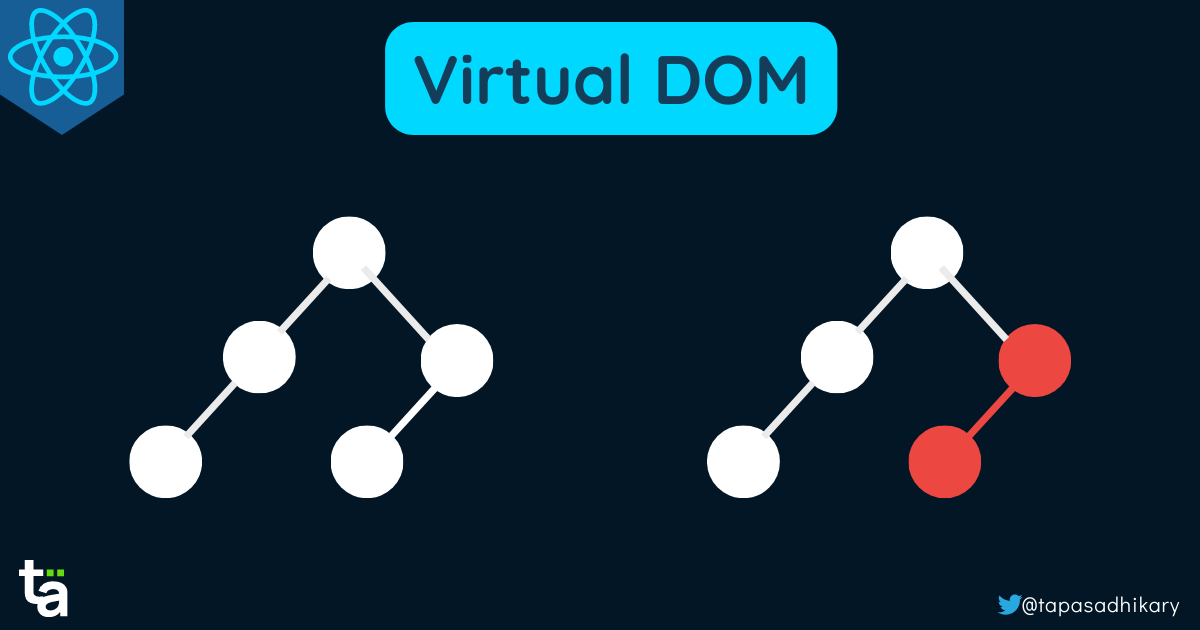
\includegraphics[height=0.3\textheight]{images/virtualDom}}
	\caption{Virtual-DOM}
\end{figure}

Das Bild zeigt schematisch, wie das Virtual DOM in React funktioniert. Zunächst wird eine virtuelle Darstellung des DOMs in Form eines Baumes erstellt. Bei Änderungen an der Benutzeroberfläche wird ein neuer Baum erstellt und mit dem vorherigen Baum verglichen. Dabei werden die Unterschiede zwischen den beiden Bäumen ermittelt. Anschließend werden nur die geänderten Elemente im tatsächlichen DOM aktualisiert. Dieser Prozess wird als Reconciliation bezeichnet \cite{ReactVirtualDOM}.

\subsubsection{Komponenten und Props}
React ist eine Bibliothek für die Entwicklung von Benutzeroberflächen, die auf dem Konzept von Komponenten und Props basiert. Eine React-Komponente ist eine eigenständige und wiederverwendbare Einheit einer Benutzeroberfläche, die entweder als Klasse oder als Funktion definiert werden kann. Komponenten können andere Komponenten enthalten und selbst als Teil einer größeren Anwendung verwendet werden \cite{ReactComponentsAndProps}.

Props (kurz für "`Properties"') sind ein wichtiger Mechanismus zur Konfiguration von React-Komponenten. Sie dienen zum Übergeben von Daten von einer Komponente zur anderen und werden als Objekt an die Komponente übergeben. Innerhalb der Komponente können Props als Parameter verwendet werden. Im Gegensatz zum State, der zur Änderung der Benutzeroberfläche innerhalb einer Komponente verwendet wird, sind Props schreibgeschützt und können nicht direkt geändert werden. Durch das Verwenden von Props können Komponenten einfach wiederverwendet werden, indem sie in verschiedenen Kontexten mit unterschiedlichen Props konfiguriert werden \cite{ReactComponentsAndProps}.

Ein Beispiel für eine React-Komponente mit Props ist die Funktion \emph{Greeting}, die einen Gruß mit dem Namen des Benutzers anzeigt. Der Name wird als Prop an die Komponente übergeben und innerhalb der Funktion als Parameter verwendet.

\newpage
Hier ist das Codebeispiel:
\begin{lstlisting}[language=vhdl,
	frame=single,           % Ein Rahmen um den Code
	framexleftmargin=15pt,  % Rahmen link von den Zahlen
	style=algoBericht,
	label={Props-Komponenten},
	captionpos=b ,          % Caption unter den Code setzen
	caption={Beispiel Kompoonente mit Probs in React}]
import React from 'react';
	
function Greeting(props) {
   return <h1>Hello, {props.name}!</h1>;
}
	
	export default Greeting;
\end{lstlisting}

Alle React-Komponenten müssen sich im Bezug auf ihre Props als sogenannte "`pure functions"' verhalten \cite{ReactComponentsAndProps}. Das bedeutet, dass die Funktion der Komponente nur von ihren Props abhängen sollte und keine weiteren Seiteneffekte haben darf. Eine Komponente, die sich wie eine "`pure function"' verhält, ist leichter zu testen und zu warten.

Es gibt auch fortgeschrittene Konzepte im Zusammenhang mit Props, wie das Konzept des "`Render Props"'. Hierbei handelt es sich um eine Technik zum Austauschen von Code zwischen React-Komponenten, bei der eine Komponente eine Funktion als Prop akzeptiert, die ein React-Element zurückgibt. Dadurch können Komponenten dynamisch wiederverwendet werden und die Codebasis der Anwendung wird vereinfacht \cite{ReactRenderProps}.

Um mit React-Komponenten und Props zu arbeiten, gibt es verschiedene Möglichkeiten. Funktionskomponenten sind die einfachste Art, eine Komponente zu definieren, indem man eine JavaScript-Funktion schreibt. Klassenkomponenten bieten mehr Funktionen, wie den Zugriff auf den State, die Möglichkeit, Lifecycle-Methoden zu definieren und vieles mehr \cite{RunebookReactComponentsAndProps}.

Insgesamt sind Komponenten und Props wichtige Konzepte in React, die Entwicklern helfen, wiederverwendbare Benutzeroberflächenkomponenten zu erstellen und die Effizienz der Entwicklung zu erhöhen.

\subsubsection{State}

In React ist der "`State"' ein Objekt, das in einer Komponente definiert wird und Werte speichert, die zur Laufzeit der Anwendung verändert werden können. Der Zustand wird in der Regel verwendet, um die Darstellung der Benutzeroberfläche zu aktualisieren, wenn sich etwas ändert. Wenn der Zustand eines Komponentenobjekts geändert wird, wird die Methode "`render()"' aufgerufen, um die Änderungen in der Benutzeroberfläche anzuzeigen \cite{W3SchoolsReactState}.

Der Zustand wird oft als Schlüssel-Wert-Paar-Objekt definiert, wobei jeder Schlüssel eine Eigenschaft repräsentiert, die geändert werden kann, und jeder Wert den aktuellen Wert dieser Eigenschaft darstellt. State-Objekte können als eine Art Konfiguration betrachtet werden, die der Komponente zur Verfügung gestellt werden, um ihre Eigenschaften und ihr Verhalten zu steuern \cite{FreeCodeCampStateInReact}.

Der Zustand ist ein beobachtbares Objekt und kann somit verändert werden. In React-Komponenten kann der Zustand durch die Verwendung der \emph{setState()}-Funktion aktualisiert werden.

Eine sorgfältige Verwaltung des Zustands in einer React-Anwendung ist wichtig, um Fehler zu vermeiden und die Leistung zu optimieren. Die Organisation des Zustands und die Datenfluss zwischen den Komponenten sollten gut durchdacht sein, um überflüssigen oder doppelten Zustand zu vermeiden \cite{ReactManagingState}.\\
Das folgende Beispiel zeigt, wie der Zustand in React-Komponenten implementiert werden kann:
\\
\begin{lstlisting}[language=vhdl,
	frame=single,           % Ein Rahmen um den Code
	framexleftmargin=15pt,  % Rahmen link von den Zahlen
	style=algoBericht,
	label={State-Fkt.},
	captionpos=b ,          % Caption unter den Code setzen
	caption={Beispiel State in Reeact}]
import React, { useState } from "react";
	
function Example() {
  // Initialisieren des State-Objekts
  const [count, setCount] = useState(0);
  //Erhoehen des Zaehlers, wenn der Button geklickt wird
  function increaseCount() {
    setCount(count + 1);
  }
	
  return (
  <div>
  <p>You clicked {count} times</p>
  <button onClick={increaseCount}>Click me</button>
  </div>
  );
 }
\end{lstlisting}

In diesem Beispiel wird die \emph{useState()} -Hook verwendet, um den Zustand der Komponente zu initialisieren. Die Funktion \emph{useState()} gibt ein Array zurück, das den aktuellen Zustand und eine Funktion zur Aktualisierung des Zustands enthält. In diesem Fall wird der Zustand mit \emph{count} initialisiert und die Funktion \emph{setCount()} wird verwendet, um den Zustand zu aktualisieren.

Beim Klick auf den Button wird die \emph{increaseCount()} Funktion aufgerufen, die den Zähler erhöht und den Zustand mithilfe von \emph{setCount()} aktualisiert. Die Änderung des Zustands löst eine erneute Ausführung der Komponente aus und die aktualisierten Werte werden in der Benutzeroberfläche angezeigt.


\subsection{Verwendung von React}
\subsubsection{Einrichtung von React}
 Eine der einfachsten Möglichkeiten, ein neues React-Projekt zu starten, ist mit einer einfachen HTML-Seite und einigen Skript-Tags \cite{deLegacyReactjs}. Dadurch ist es möglich in kürzester Zeit eine Grundeinstellung erstellen.
 
 Eine andere Möglichkeit, mit der Entwicklung von React-Anwendungen zu beginnen, bietet der \emph{Create-React-App}-Generator \cite{vsCodeReactTutorial}.Der Generator ist eine schnelle und einfache Möglichkeit, neue React-Projekte einzurichten. Um den Generator zu verwenden, wird der folgende Befehl im Terminal ausgeführt:
 
\begin{lstlisting}[language=vhdl,
	frame=single,           % Ein Rahmen um den Code
	framexleftmargin=15pt,  % Rahmen link von den Zahlen
	style=algoBericht,
	label={App-Erstellung},
	captionpos=b ,          % Caption unter den Code setzen
	caption={Beispiel Anwendungserstellung}]
npx create-react-app my-app
cd my-app
npm start
\end{lstlisting}
Durch Ausführen von \emph{npx create-react-app my-app} wird ein neues React-Projekt mit dem Namen \emph{my-app} erstellt. Mit \emph{cd my-app} wird in das neu erstellte Verzeichnis gewechselt. Anschließend wird die Anwendung mit dem Befehl\emph{npm start} gestartet.
Der Webserver startet und die Anwendung ist unter \emph{http://localhost:3000} im Browser aufrufbar.

React wurde entwickelt, um keine Annahmen über den Rest des Technologie-Stacks zu treffen. So ist es möglich neue Features zu entwickeln, ohne bestehenden Code umzuschreiben \cite{deLegacyReactjsDocs}. React kann auf dem Server mit Node oder als mobile Anwendung mit React Native gerendert werden.

Zusammenfassend lässt sich sagen, dass die Einrichtung von React ein unkomplizierter Prozess ist, mit dem es möglich ist in kurzer Zeit mit der Entwicklung von Benutzeroberflächen für Web- und mobile Anwendungen zu beginnen.

\subsubsection{Komponentenentwicklung}
Die Entwicklung von Komponenten ist ein wichtiger Aspekt bei der Verwendung von React. React-Komponenten sind wiederverwendbare Elemente, die das Erstellen von Benutzeroberflächen erleichtert. Eine React-Komponente implementiert eine \emph{render()}-Methode, die Eingabedaten (Props) nimmt und zurückgibt, was gerendert wird. Es verwendet eine XML-ähnliche Syntax namens JSX, mit der es HTML-ähnlichen Code direkt in JavaScript schreiben kann. \cite{deLegacyReactjs}

Ein einfaches Beispiel für eine React-Komponente ist ein "`Gruß"' (Greeting) Komponente, die eine Begrüßungsnachricht basierend auf dem übergebenen Namen anzeigt:
\begin{lstlisting}[language=vhdl,
	frame=single,           % Ein Rahmen um den Code
	framexleftmargin=15pt,  % Rahmen link von den Zahlen
	style=algoBericht,
	label={Greeting-Komponente},
	captionpos=b ,          % Caption unter den Code setzen
	caption={Beispiel Komponentenentwicklung }]
import React, { Component } from 'react';

class Greeting extends Component {
     render() {
        const { name } = this.props;
        return <h1>Hallo, {name}!</h1>;
    }
}
\end{lstlisting}
In diesem Beispiel wird eine Greeting-Komponente erstellt, die die \emph{render()}-Methode implementiert. Auf die übergebenen Eingabedaten, welche an die Komponente übergeben werden, ist es mittels \emph{this.props} möglich darauf zuzugreifen \cite{deLegacyReactjs}. Mit der JSX-Syntax wird eine Willkommensnachricht direkt in ein HTML-ähnliches Element einfügen.

React fördert einen Komponentenentwicklungsansatz, um modulare, wiederverwendbare Benutzeroberflächen zu erstellen. Die Aufteilung der Benutzeroberfläche in kleinere Komponenten erleichtert die Organisation und Wartung des Codes.

\subsubsection{Ereignisbehandlung}
Die Ereignisbehandlung ist ein weiterer wichtiger Aspekt bei der Verwendung von React. Dadurch ist es möglich auf Benutzeraktionen wie Klicks und Tastenanschläge zu reagieren und die Anwendung entsprechend zu aktualisieren. Bei React-Elementen ist die Ereignisbehandlung ähnlich wie bei DOM-Elementen, es gibt jedoch einige syntaktische Unterschiede.

Beispielsweise werden die Ereignisse von React in CamelCase statt in Kleinbuchstaben benannt, und JSX übergibt Funktionen als Event-Handler anstelle von Strings. \cite{react_de_handling_events}

Ein einfaches Beispiel für die Ereignisbehandlung in React ist eine Schaltfläche (Button), die bei einem Klick eine Nachricht in der Konsole ausgibt:

\begin{lstlisting}[language=vhdl,
	frame=single,           % Ein Rahmen um den Code
	framexleftmargin=15pt,  % Rahmen link von den Zahlen
	style=algoBericht,
	label={Events},
	captionpos=b ,          % Caption unter den Code setzen
	caption={Beispiel EventHandler}]
import React, { Component } from 'react';

class ButtonClick extends Component {
     handleClick() {
         console.log('Button wurde geklickt!');
     }
 
 render() {
 	return (
 	    <button onClick={this.handleClick}>
 	    Klick mich!
 	    </button>
 	    );
     }
 }

\end{lstlisting}

In diesem Beispiel wird eine \emph{ButtonClick} Komponente erstellt, die die \emph{render()} Methode implementiert und ein \emph{<button>} Element mit einem \emph{onClick Eventhandler} zurückgibt. Der Eventhandler ist die \emph{handleClick} Methode, die in der Komponente definiert ist. Wenn der Benutzer auf den Button klickt, wird die \emph{handleClick} Methode ausgeführt und die Nachricht "`Button wurde geklickt!"' in der Konsole angezeigt. \cite{react_de_handling_events}

Die Ereignisbehandlung in React ermöglicht es, interaktive Benutzeroberflächen zu erstellen und auf Benutzeraktionen dynamisch zu reagieren. Durch die Verwendung von Eventhandlern können Anwendungen auf Benutzerinteraktionen reagieren und den Zustand der Anwendung und die Benutzeroberfläche entsprechend aktualisieren.

\subsubsection{JSX}
JSX ist eine XML-ähnliche Syntax, die von React verwendet wird, um die Benutzeroberfläche einer Anwendung zu definieren \cite{deLegacyReactjs}. JSX ermöglicht es Entwicklern, die Struktur und das Erscheinungsbild von Komponenten ähnlich wie HTML zu beschreiben. Die Verwendung von JSX ist optional, hat sich jedoch als effizient und bequem für die Arbeit mit React-Komponenten erwiesen.

In JSX werden Komponenten als Tags definiert, die HTML-Tags ähneln, mit einigen Unterschieden. Zum Beispiel behandelt React Komponenten in Kleinbuchstaben als DOM-Tags und Komponenten in Großbuchstaben als benutzerdefinierte Komponenten \cite{ReactComponentsAndProps}. Dies bedeutet, dass \emph{<div />} ein HTML div-Tag darstellt, während \emph{<Welcome />} eine benutzerdefinierte React-Komponente darstellt, vorausgesetzt, dass \emph{Welcome} im Scope ist.

JSX bietet auch die Möglichkeit, JavaScript-Ausdrücke in die Komponentenstruktur einzubetten, indem sie in geschweiften Klammern {} eingeschlossen werden. Diese Ausdrücke können Variablen, Funktionen oder Berechnungen enthalten, die zur Laufzeit ausgewertet werden.

Ein weiterer Aspekt von JSX ist das Übergeben von Daten an Komponenten mit Hilfe von Eigenschaften. Props können in JSX wie HTML-Attribute definiert werden und schließen bei JavaScript-Ausdrücken den Wert in geschweiften Klammern ein \cite{deLegacyReactjs}. Innerhalb der Komponente sind diese Props über this.props zugänglich.\\
Ein Beispiel für eine React-Komponente mit JSX:
\\
\begin{lstlisting}[language=vhdl,
	frame=single,           % Ein Rahmen um den Code
	framexleftmargin=15pt,  % Rahmen link von den Zahlen
	style=algoBericht,
	label={JSX},
	captionpos=b ,          % Caption unter den Code setzen
	caption={Beispiel JSX }]
class Welcome extends React.Component {
        render() {
        	return <h1>Hallo, {this.props.name}!</h1>;
        }
    }

    ReactDOM.render(
    <Welcome name="Max" />,
    document.getElementById('root')
    );
\end{lstlisting}
In diesem Beispiel wird eine benutzerdefinierte React-Komponente namens \emph{Welcome} erstellt, die einen Namen über Props erhält und eine Begrüßungsnachricht mit dem Namen anzeigt.

Insgesamt ist JSX eine leistungsstarke Syntax, die die Arbeit mit React-Komponenten erleichtert und die Entwicklung von Anwendungen effizienter gestaltet. Es ermöglicht Entwicklern, die Struktur ihrer Anwendung auf eine Weise zu definieren, die sowohl intuitiv als auch leicht verständlich ist.

\subsection{Fortgeschrittene Themen in React}
React bietet eine Vielzahl von fortgeschrittenen Techniken und Bibliotheken, um komplexe Anwendungen zu entwickeln. Einige dieser Techniken sind Redux oder Context API, React Router, React Hooks und serverseitiges Rendern.

\subsubsection{Redux oder Context API}
React Redux und Context API sind zwei beliebte Bibliotheken, die React-basierte Anwendungen für das Datenflussmanagement verwenden können. Beide Bibliotheken dienen dem Zweck, den Zugriff auf Daten zu vereinfachen und den Anwendungsstatus effektiv zu verwalten.

Redux ist eine Bibliothek, die den Anwendungszustand in einem zentralen Speicher speichert. Dies vereinfacht den Zugriff auf den Anwendungsweiten Status und macht den Gesamtcode strukturierter. Redux bietet auch die Möglichkeit, den Status zu ändern, indem Aktionen ausgelöst werden, die den Status aktualisieren. \cite{scalablepath} \\
Die folgende Abbildung zeigt das Datenmanagement in Redux:
\begin{figure}[htbp]
	\centering
	\fbox{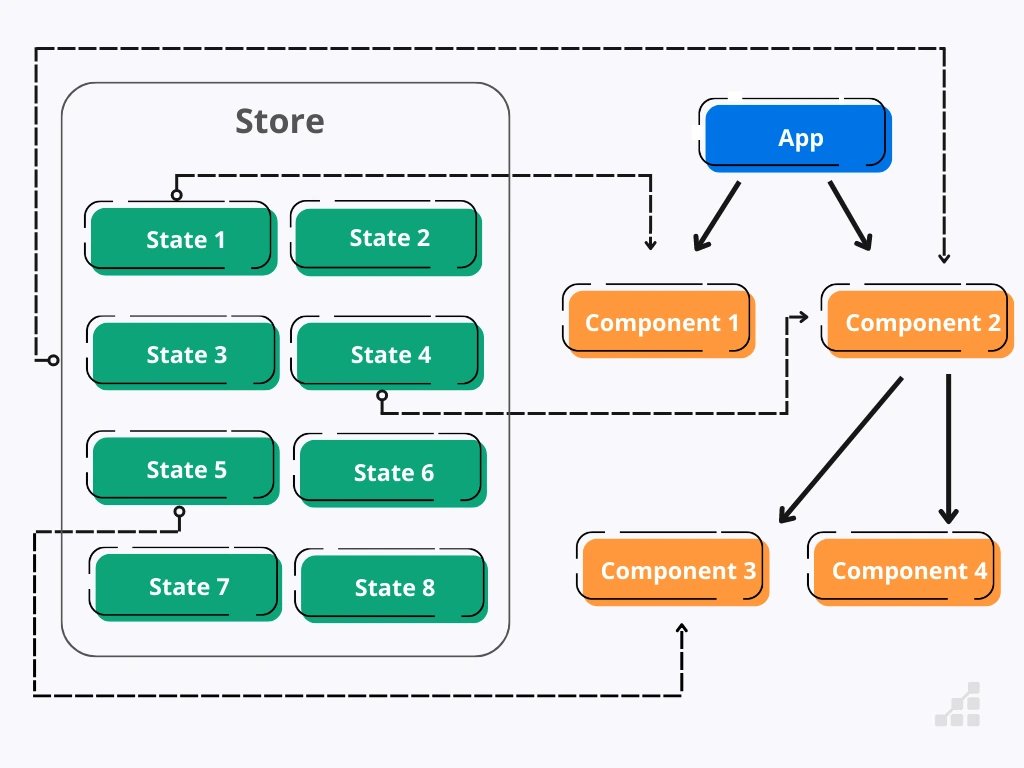
\includegraphics[height=0.3\textheight]{images/redux}}
	\caption{Redux-Datenfluss}
\end{figure}\\
Der Zustand der Anwendung wird im Store gespeichert, der die Datenstruktur und die aktuellen Daten enthält. Die Komponenten erhalten den Zugriff auf den Zustand über das Connect-Modul, das es ihnen ermöglicht, auf die Daten zuzugreifen und sie in ihre Eigenschaften zu übertragen. Wenn ein Ereignis eintritt, das den Zustand ändert, wird eine Action ausgelöst, die eine Reducer-Funktion aufruft, um den Zustand im Store zu aktualisieren.

Redux eignet sich besonders für Anwendungen mit vielen Komponenten und komplexen Datenstrukturen. Der Hauptvorteil von Redux besteht darin, dass das Datenflussmanagement einheitlich und leicht verständlich ist. Dies vereinfacht die Anwendungswartung erheblich, da Entwickler immer genau wissen, wo ihr Anwendungsstatus gespeichert ist und wie sie darauf zugreifen können.

Die Kontext-API ist eine Redux-Alternative, mit der Entwickler den Status in ihrer Komponentenhierarchie verwalten können. Die Kontext-API erleichtert den Zugriff auf den Status, indem sie ermöglicht, dass er in der gesamten Komponentenhierarchie weitergegeben wird. Im Gegensatz zu Redux ist die Context-API jedoch nicht gut für Anwendungen mit komplexen Datenstrukturen und vielen Komponenten geeignet. \cite{scalablepath} \\
Die folgende Abbildung zeigt den Datenfluss in Context API:
\begin{figure}[htbp]
	\centering
	\fbox{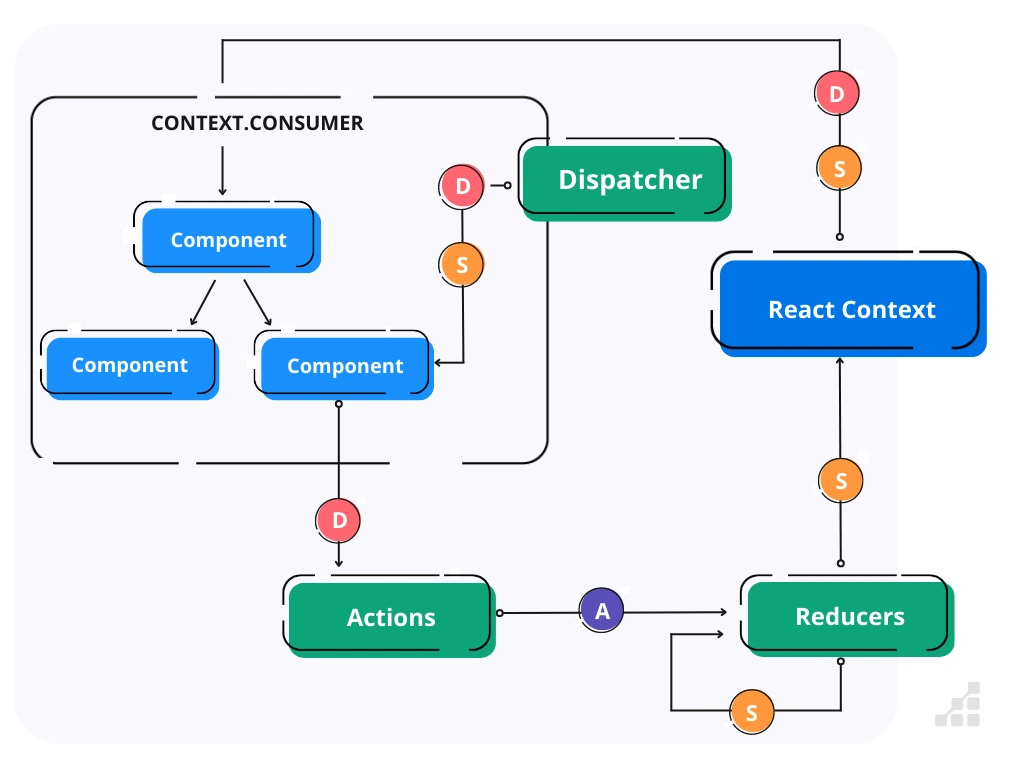
\includegraphics[height=0.3\textheight]{images/context-api}}
	\caption{ContextApi-Datenfluss}
\end{figure}\\
Der Zustand wird in einer höheren Komponente gespeichert und durch die Prop-Drilling-Technik an untergeordnete Komponenten übermittelt. Dadurch können untergeordnete Komponenten den Zustand der höheren Komponenten ändern und somit auch den Zustand der Anwendung beeinflussen.

Die Kontext-API eignet sich am besten für Anwendungen, bei denen der Zustand nicht zu komplex und die Anzahl der Komponenten begrenzt ist. Der Hauptvorteil der Kontext-API besteht darin, dass sie eine einfachere und schnellere Möglichkeit bietet, auf den Status zuzugreifen, ohne einen globalen Speicher einrichten und verwalten zu müssen. \cite{scalablepath}

Insgesamt eignet sich Redux für große Anwendungen mit vielen Komponenten und komplexen Datenstrukturen, während die Context-API für kleine Anwendungen mit einer begrenzten Anzahl von Komponenten und einem einfachen Datenmodell geeignet ist. Beide Bibliotheken sind jedoch nützliche Tools für ein effektives Datenflussmanagement in React-basierten Anwendungen. \cite{scalablepath}


\subsubsection{React Router}
React Router ist eine JavaScript-Bibliothek, die in Verbindung mit der React-Bibliothek verwendet wird.Es ermöglicht eine effiziente und reibungslose Navigation zwischen verschiedenen Seiten oder Komponenten innerhalb einer Webanwendung.
Die Verwendung von React Router bringt viele Vorteile für das Design und die Entwicklung von Webanwendungen.

Erstens können Inhalte dynamisch angezeigt werden, ohne die gesamte Seite neu zu laden. Dies sorgt für eine schnellere und einfachere Erfahrung für Endbenutzer. Zweitens trägt es dazu bei, das Layout der Anwendung sauber und gut strukturiert zu halten, indem es die Navigation zwischen den verschiedenen Komponenten einer Anwendung erleichtert.

React Router verwendet eine hierarchische Struktur, um die Navigation innerhalb der Anwendung zu organisieren.Dazu können mehrere Unterthemen bzw. Komponenten zu einem Oberthema bzw. Hauptkomponente zusammengefasst und für jedes dieser Unterthemen unterschiedliche Routen definiert werden.

Auf diese Weise können Entwickler ihre Anwendungen modularisieren und gleichzeitig ihre Wartbarkeit und Skalierbarkeit sicherstellen.

Um React Router in einer React-Anwendung zu verwenden, muss zuerst die React-Router-Dom-Bibliothek installiert werden. Dies kann durch Ausführen des Befehls \emph{npm i -D respond-router-dom} in einem Terminal im Stammverzeichnis der Anwendung erreicht werden.Anschließend ist es möglich mit React Router verschiedene Routen und Komponenten zu definieren und zu verknüpfen, um eine effiziente und benutzerfreundliche Navigation innerhalb einer Anwendung zu gewährleisten.

Zusammenfassend ist React Router eine praktische und weit verbreitete Bibliothek, mit der es möglich ist eine effiziente Navigation und Routenverwaltung in einer React-Anwendungen implementieren zu können. So eine einfach zu integrierende und modulare Struktur ermöglicht es Entwicklern, schnell und einfach attraktive und einfach zu bedienende Webanwendungen zu erstellen. \cite{react-router}

\subsubsection{React Hooks}
React Hooks ist eine revolutionäre Funktion, welche in React Version 16.8.0 eingeführt wurde. Es ist Entwicklern möglich, Status- und andere React-Funktionen in funktionalen Komponenten zu verwenden, ohne Klassenkomponenten schreiben zu müssen..

React Hooks haben gegenüber Klassenkomponenten einige Vorteile. Zu mal ist die Syntax einfacher und leichter  zu verstehen, wodurch Ihr Code leichter zu lesen und zu warten ist. Zudem erleichtert es die gemeinsame Nutzung von Logik zwischen Komponenten, ohne dass komplexe Entwurfsmuster wie Komponenten höherer Ordnung und Render-Props erforderlich sind.

Die in React verfügbaren grundlegenden Hooks sind die Hooks \emph{useState} und \emph{useEffect}. Mit dem \emph{useState}-Hook können Sie den lokalen Status funktionaler Komponenten verwalten und aktualisieren. Der \emph{useEffect}-Hook hingegen wird in funktionalen Komponenten verwendet, um Seiteneffekte wie Datenabruf und Ereignisabonnements zu behandeln.

Um Hooks in einer React-Anwendung zu verwenden, müssen die entsprechenden Hooks zuerst aus der React-Bibliothek importiert werden. Diese Hooks können dann innerhalb funktionaler Komponenten verwendet werden, um den gewünschten Zustand oder Nebeneffekte zu verwalten. Es ist wichtig zu beachten, dass Hooks nur innerhalb von Funktionskomponenten verwendet werden können, nicht innerhalb von Klassenkomponenten oder JavaScript-Funktionen. \cite{react-hooks}

Zusammenfassend sind React Hooks eine leistungsstarke und innovative Funktion, die es Entwicklern ermöglicht, den Status von Funktionskomponenten und anderen React-Funktionen effizient zu verwalten. React Hooks verändern und vereinfachen grundlegend die Art und Weise, wie React-Anwendungen entwickelt werden, indem sie eine einfache Integration und verbesserte Code-Lesbarkeit bieten.

\subsubsection{Serverseitiges Rendern}
Serverseitiges Rendering (SSR) ist ein wichtiger Aspekt der React-Anwendungsentwicklung, der es ermöglicht, React-Komponenten auf dem Server zu rendern, bevor das vollständig gerenderte HTML-Dokument an den Client gesendet wird.
Die Herausforderung beim Erstellen von Webanwendungen besteht darin, ein optimales Benutzererlebnis zu gewährleisten und gleichzeitig die Sichtbarkeit in Suchmaschinen zu erhöhen. Serverseitiges Rendering bietet hierfür eine Lösung.

\begin{figure}[htbp]
	\centering
	\fbox{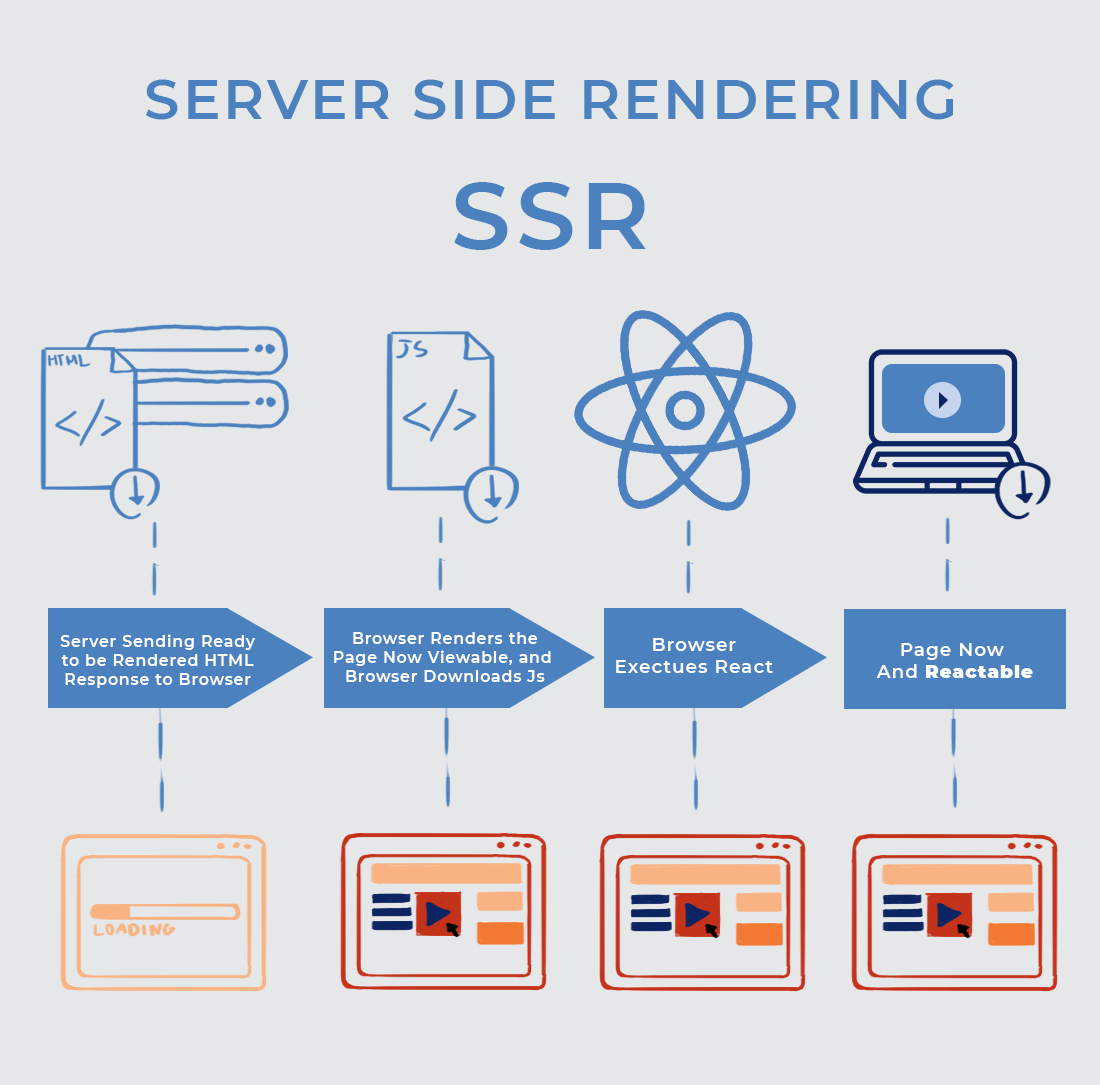
\includegraphics[height=0.3\textheight]{images/ssr}}
	\caption{SSR in React}
\end{figure}
Der Prozess des serverseitigen Renderns in React kann in vier Schritten zusammengefasst werden, wie im angegebenen Bild dargestellt:\\
\begin{itemize}
	\item[1.] {Der Client sendet eine HTTP-Anfrage an den Server}
	\item[2.]  {Der Server rendert die React-Komponenten der Seite in einen HTML-String.}
	\item[3.]  {Der Server injiziert den gerenderten HTML-String in ein HTML-Dokument.}
	\item[4.]  {Der Server sendet das vollständig gerenderte HTML-Dokument an den Client.}
\end{itemize}
Um serverseitiges Rendering in einer React-Anwendung zu implementieren, muss ein eigener Backend-Server entwickelt werden. Die Serverintegration von Node.js ist in diesem Zusammenhang eine gängige Lösung. Darüber hinaus sind möglicherweise weitere Anpassungen erforderlich, z. B. die Verwendung von serverseitigem Rendering mit React Router. \cite{Drehmanns2021}

Zusammenfassend lässt sich sagen, dass serverseitiges Rendering eine nützliche Technik zur Verbesserung der Leistung und Suchmaschinenoptimierung von React-Anwendungen ist. Indem Sie Ihre Anwendung auf dem Server rendern und das vollständig gerenderte HTML-Dokument an den Client senden, können Sie die anfänglichen Ladezeiten verkürzen und die Sichtbarkeit Ihrer Anwendung in Suchmaschinen erhöhen.

\subsection{Best Practices in React-Entwicklung}
 Bei der Entwicklung von React-Anwendungen ist es entscheidend, bewährte Methoden und Best Practices einzuhalten, um skalierbare, wartbare und effiziente Anwendungen zu erstellen. Einige dieser Best Practices beziehen sich auf das Verwenden von Werkzeugen und Bibliotheken, die die Produktivität steigern und die Codequalität verbessern. 
\subsubsection{Testen von React-Anwendungen}
Das Testen von React-Anwendungen ist ein wichtiger Aspekt, um die Codequalität und Zuverlässigkeit in der Softwareentwicklung sicherzustellen. Es gibt verschiedene Testmethoden und Tools, die auf verschiedene Aspekte einer Anwendung abzielen.
\begin{figure}[htbp]
	\centering
	\fbox{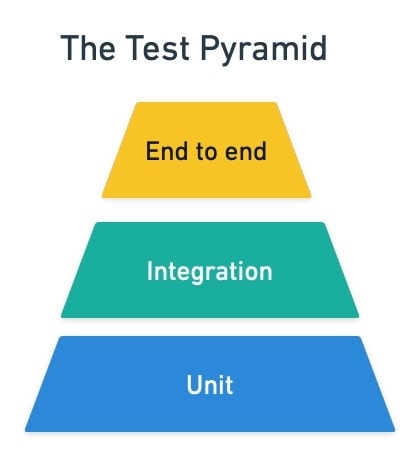
\includegraphics[height=0.3\textheight]{images/pyramid}}
	\caption{Test Pyramid}
\end{figure}
Die oben abgebildete Testpyramide ist ein Konzept, welches zur Erstellung verschiedener Testmethoden hilft.Dazu gehören End-to-End-Tests (E2E), Integrationstests und Komponententests (Unit-Tests). Unit-Tests werden für kleine, isolierte Codeblöcke wie einzelne Funktionen oder Komponenten verwendet und konzentrieren sich auf das Testen von Teilaspekten der Anwendung.

Ein beliebtes Tool zum Testen von React-Anwendungen ist die React Testing Library (RTL). RTL konzentriert sich darauf, die Komponente aus der Sicht des Endbenutzers zu testen, anstatt die Implementierung und Logik der zugrundeliegenden React-Komponente zu validieren. Auf diese Weise können Entwickler sicherstellen, dass ihre Anwendungen für ihre Benutzer wie erwartet funktionieren. \cite{react-test-runebook}

Jest ist ein weiteres beliebtes Testtool, das speziell zum Testen von React-Anwendungen entwickelt wurde. Es ordnet und strukturiert die Testsuite und überprüft die gewünschten Eigenschaften. In Kombination mit Enzyme, das den zu testenden Frontend-Code ausführt und die relevanten Schnittstellen bereitstellt, ermöglicht Jest Entwicklern den Zugriff auf und die Interaktion mit den generierten Elementen. \cite{react-test-ix}

Zusammenfassend lässt sich sagen, dass das Testen von React-Anwendungen ein wichtiger Teil des Entwicklungsprozesses ist, der dazu beiträgt, die Codequalität sicherzustellen und potenzielle Fehler frühzeitig zu erkennen. Durch die Verwendung von Testwerkzeugen wie der React Testing Library und Jest in Verbindung mit den Prinzipien der Testpyramide können Entwickler umfassende Tests durchführen, um sicherzustellen, dass sich ihre Anwendungen wie erwartet verhalten.

\subsubsection{Performance-Optimierung}
Die Performance-Optimierung ist ein Schlüsselfaktor bei der Entwicklung von React-Anwendungen, um eine schnelle und reaktionsschnelle Benutzererfahrung zu erreichen. Es gibt verschiedene Ansätze und Techniken, um die Leistung von React-Anwendungen zu optimieren.

Eine gängige Methode zur Verbesserung der Leistung in React ist die Verwendung von \emph{React.PureComponent}. Anstatt ein eigenes \emph{shouldComponentUpdate} zu schreiben, ist es möglich \emph{React.PureComponent} zu verwenden, um unnötiges Rendern von Komponenten zu verhindern. \emph{React.PureComponent} führt einen flachen Vergleich von Props und State durch. In vielen Fällen reicht dies aus, um unnötige Updates zu vermeiden.
Es ist jedoch wichtig zu beachten, dass \emph{React.PureComponent} möglicherweise nicht geeignet ist, wenn Props oder State auf eine Weise mutiert werden, die bei einem oberflächlichen Vergleich übersehen würde.

Neben der Verwendung von \emph{React.PureComponent} ist es wichtig, die Gesamtleistung der Webanwendung zu berücksichtigen. Beispielsweise kann die Optimierung von CSS-Dateien einen erheblichen Einfluss auf die Anwendungsleistung haben. In einem Testfall benötigte der Browser über 50 ms, um die zweite doppelt eingebettete CSS-Datei von 25 KiB zu interpretieren und die Regeln korrekt anzuwenden, während die erste Datei nur 6 ms brauchte. Dies unterstreicht, wie wichtig es ist, Ressourcen sorgfältig zu verwalten und unnötige Doppelarbeit zu vermeiden. \cite{react-performance}

Insgesamt ist die Optimierung der Leistung einer React-Anwendung ein wichtiger Aspekt, um eine schnelle und reaktionsschnelle Benutzererfahrung sicherzustellen. Die Verwendung von Techniken wie \emph{React.PureComponent} und die Optimierung von Ressourcen wie CSS-Dateien können die Anwendungsleistung verbessern und die beste Benutzererfahrung gewährleisten. \cite{css-performance}


\subsubsection{Sicherheit und React}
Wenn es um Sicherheit geht, bietet React einige integrierte Funktionen, um häufige Web-Sicherheitsprobleme zu vermeiden. Allerdings liegt es auch in der Verantwortung des Entwicklers, für die Sicherheit der Anwendung zu sorgen.

React rät beispielsweise von der Verwendung unsicheren Codes ab, indem es JSX bereitstellt, das Ausdrücke vor dem Rendern standardmäßig maskiert, um Cross-Site-Scripting-Angriffe (XSS) zu verhindern. Es soll jedoch beachtet werden, dass ReactJS selbst keine vollständige Sicherheitslösung ist. Auch auf andere Sicherheitsaspekte wie sichere API-Endpunkte und den richtigen Einsatz von HTTPS sollten Entwickler bewusst achten.

Darüber hinaus gibt es Tools wie "`Invicti Web Application Security Scanner"', die automatische Schwachstellenprüfungen durchführen und dabei helfen, die Sicherheit von React-Anwendungen weiter zu verbessern \cite{geekflare_learning_resources} \cite{geekflare_rendering}.

Insgesamt bietet React eine solide Grundlage für die sichere Entwicklung von Webanwendungen, erfordert jedoch von den Entwicklern dennoch ein hohes Maß an Bewusstsein und Sorgfalt, um sicher zu stellen, dass ihre Anwendungen resistent gegen Angriffe sind.

\subsection{Vergleich mit anderen Frontend-Technologien}
In diesem Kapitel werden die unterschiedlichsten Frontend- Technologien miteinander verglichen.
\subsubsection{Vor- und Nachteile von React im Vergleich zu Angular und Vue.js}
React, Angular und Vue.js sind beliebte Frontend-Technologien, die bei der Entwicklung von modernen Webanwendungen eingesetzt werden. Jede Technologie hat ihre Vor- und Nachteile, die bei der Wahl der Technologie berücksichtigt werden sollten.
Angular, React und Vue.js sind alle weit verbreitet und haben jeweils ihre Stärken und Schwächen.

Angular ist ein umfangreiches Framework zum Erstellen skalierbarer und leistungsstarker Anwendungen. Es verfügt über einen schlanken Kerncode mit hoher Modularität mit externen Komponenten, was eine unbegrenzte Integration und Nutzung von HTML und CSS ermöglicht. Darüber hinaus unterstützt es TypeScript und JavaScript und trennt Vorlagen strikt von Design und Logik \cite{hosttest2021}. Der Nachteil ist, dass frühere Angular-Versionen nicht gut für den Aufbau dynamischer Webanwendungen und komplexer digitaler Produkte geeignet sind \cite{ichi2023}.

React hingegen ist eine Open-Source-GUI-Bibliothek und bietet einige Vorteile. Neue Entwickler können dieses Tool leicht erlernen. Es kann mit anderen JS-Bibliotheken und Frameworks verwendet werden \cite{softwaredeveloperindia2022}. React verfügt außerdem über eine sehr aktive Community, die ständig neue Bibliotheken und Tools entwickelt, um die Entwicklung einfacher und schneller zu machen. Der Nachteil ist, dass es nicht so leistungsstark ist wie Angular oder Vue \cite{logrocket2021}.

Vue.js ist dasjenige neueste der drei Frameworks und zeichnet sich durch eine einfache Satzlehre und eine leichte Lernkurve aus. Es hat eine sehr schnelle Startzeit und ist daher unter Entwicklern beliebt, selbige schnell Prototypen hinstellen möchten \cite{logrocket2021}. Obwohl Vue.js eine kleinere Community hat denn Angular und React, wächst jene schnell und bietet eine starke Unterstützung \cite{codeinwp}.

Diese Vor- und Nachteile werden in der nachfolgenden Tabelle nochmals visualisiert.
\begin{center}
\begin{table}[h]
	\begin{tabularx}{4cm}{|l|l|p{4.5 cm}|ll}
		\cline{1-3}
		\textbf{Technolgie} & \textbf{Vorteil}                         & \textbf{Nachteil}                                                &  &  \\ \cline{1-3}
		Angular             & Schlanker Kerncode mit hoher Modularität & nicht geeignet für dynamiche Web-App  &  &  \\ \cline{1-3}
		React               & Einfach zu erlernen, aktive Community    & Weniger leistungsstark         &  &  \\ \cline{1-3}
		Vue.js              & Einfache Satzlehre, schnelle Startzeit   & Kleinere Community             &  &  \\ \cline{1-3}
	\end{tabularx}
\end{table}
\end{center}

Zusammenfassend haben alle drei Frameworks ihre eigenen Stärken und Schwächen und die Wahl hängt deutlich von den spezifischen Erwartungen und Präferenzen des Entwicklerteams ab.

\subsection{Fazit}
React hat sich als eine der beliebtesten JavaScript-Bibliotheken etabliert und bietet Entwicklern eine effiziente und flexible Plattform zum Erstellen von Benutzeroberflächen für Webanwendungen. Es zeichnet sich durch die Bereitstellung wiederverwendbarer UI-Komponenten und einer deklarativen Codestruktur aus, die das Debuggen und die Vorhersagbarkeit erleichtert.

Die Weiterentwicklung von React zeigt deutlich, dass der Trend zur Verwendung von React Hooks weiter zunimmt. Sie bieten eine einfachere und effizientere Möglichkeit zur Erstellung von React-Komponenten und werden bereits von vielen Unternehmen in der Produktion eingesetzt. Es wird erwartet, dass dieser Trend die Zukunft der React-Entwicklung prägen wird. React lebt in einem dynamischen Ökosystem und interagiert mit anderen Technologien und Frameworks. Neuere Technologien wie Svelte verfolgen einen anderen Ansatz bei der Nutzung des virtuellen DOM und könnten zu zukünftigen Verbesserungen und Änderungen an React führen.

Zusammenfassend lässt sich sagen, dass React aufgrund seiner Flexibilität, Beliebtheit und aktiven Community eine starke Position in der Zukunft der Webentwicklung einnehmen könnte. Es wird erwartet, dass React seine Rolle als Branchenführer beibehält und weiterhin innovative Lösungen für die Entwicklung von Benutzeroberflächen bereit stellt.

\section{Docker}

\begin{wrapfigure}{r}{0.4\textwidth}
	\centering
	\fbox{
\includegraphics[width=0.30\textwidth]{images/docker}}
\end{wrapfigure}

Docker ist eine Open Source Container basierte Virtualisierungssoftware von Docker.inc.
Sie kann eine Software mit all ihren benötigten Abhängigkeiten (z.B. Bibliotheken) in ein Docker-Image packen. Dieses Image kann Docker unabhängig von der Plattform oder der vorhandenen Software in einen sogenannten Container (Sandbox) ausführen. Dadurch ist er von anderen Prozessen auf dem Host-System isoliert. Die Kommunikation zwischen den Containern läuft deswegen meistens über eine Netzwerk-API.

Dies ermöglicht einen hohen Grad an Flexibilität, erhöht die Sicherheit und verhindert Probleme mit verschiedenen Versionen von Bibliotheken oder Software.

\cite{dockerDummies}
\cite{dockerOverview}

\subsection{Docker-Daemon}
Der Kern von Docker ist der Docker-Daemon. Er verwaltet die Container und wird per Docker-Engine ( API) gesteuert. Dazu gibt es verschiedene Programme, die Clients genannt werden. Je nach Aufgabe kann ein Client besser geeignet sein als ein anderer. Es muss sich aber nicht auf einen festgelegt werden. Auch die parallele Nutzung ist möglich. In diesem Projekt kommen Docker und Compose zum Einsatz.
\cite{dockerDaemon}
\cite{dockerDaemon}

\subsection{Docker Images und Container}
Ein Docker-Image bildet die Grundlage für jeden Container. Wie bei einem Bauplan besteht es aus einer Liste von Änderungen in einer festen Reihenfolge.

Beim Starten eines Containers werden diese Änderungen in dem virtuelle Dateisystem des Container ausgeführt. Somit kann ein Programm mitsamt Daten und Bibliotheken in einem Container laufen.

Für die Kommunikation hat Docker Container-Netzwerke. Im Standardfall stellt Docker drei Netzwerke bereit und sofern nicht anders eingestellt, wird jeder Container in das \emph{Docker0} Netzwerk eingebunden. Damit er auch von außerhalb erreichbar ist, muss beim Start des Containers eine Portweiterleitung angegeben werden.\\
In der Praxis ist der Ablauf folgendermaßen: \\
1. Ein Docker-Image mit dem Programm und dazugehörigen Daten erzeugen. \\
2. Image als Container starten. \\
Um ein Image zu erstellen wird meist ein vorhandenes Docker-Image als Basis verwendet. \emph{www.dockerhub.com} bietet eine Vielzahl an Images für alle möglichen Anwendungen an.
In einer Datei mit den Namen Dockerfile kann mit \emph{FROM "`imagename"'} eins der Images einfach als Basis festgelegt werden. Danach können eigene Dateien kopiert oder Programme installiert bzw. ausgeführt werden.

Beim Starten eines Containers können Konfigurationen festgelegt werden (z.B. Portweiterleitung).
Jedes Image kann beliebig oft als Container mit eigenen Einstellungen gestartet werden. So ist es möglich, das selbe Image mit unterschiedlicher Konfiguration gleichzeitig laufen zu lassen.

Zudem können Umgebungsvariablen definiert werden, die Docker beim Start des Containers übernimmt. Somit können Einstellungen und Daten für die Software im Container bereitgestellt werden, ohne das Docker-Image ändern zu müssen.

\cite{dockerDummies}

\subsection{Docker Compose }
Gehören zu einer Anwendung oder einem Service mehrere Container so bietet der Client \emph{Docker Compose} die Möglichkeiten automatisch Images zu erzeugen und Container zu starten. Dieser muss meist erst installiert werden.

Für \emph{compose} wird eine \emph{compose.yaml} Datei verwendet. In dieser stehen die  zu startenden Container und die jeweils dazugehörige Konfiguration.
Mit dem Befehl \emph{docker compose up} starten alle Container.
Dadurch wird ein vollautomatisierter Arbeitsprozess ermöglicht.

\subsection{Vor- und Nachteile von Docker }
Docker ermöglicht durch seine flexible Abstraktion einen fast plattformunabhängigen Betrieb von Software. Dies wird erreicht in dem Docker verschiedene Ebenen von Abstraktionen verwendet um so für die Software eine einheitliche Umgebung zu gewährleisten. Es wird aber im Gegensatz zu virtuellen Maschinen keine Hardware simuliert.

Für die Abstraktion werden allerdings mehr Ressourcen benötigt, da teilweise ganze Betriebssysteme in einem Container laufen. Somit kann ein einzelner Docker Container gern mal mehrere GB an Arbeitsspeicher benötigen.

Zudem kann das bauen eines Containers je nach Rechenleistung und Internetgeschwindigkeit einiges an Zeit in Anspruch nehmen. Das kann vor allem beim Entwickeln viel Zeit kosten, wenn zum Testen der Container mehrmals hintereinander neu gebaut werden müssen.

\cite{dockerDummies}
\cite{dockerComposeOverview}

\subsection{Docker unter Windows }
Um Docker unter Windows benutzen zu können muss WSL2 (Windows Subsystem for Linux 2) installiert und aktiviert sein.
In diesem läuft dann der Docker-Daemon.

Docker Desktop ist ein Client mit Grafischer Oberfläche. Dieser steuert den Docker-Dienst um Container zu starten oder zu stoppen.

Nach dem Start zeigt er die Container welche Docker gespeichert hat mit Namen, Images, Ports und wann er zuletzt gestartet wurde. (Abb: \ref{fig-docker-desktop})
Mit einem Klick auf den Container können unter anderem seine Logs oder ein Terminal im Container erreicht werden, welche bei der Fehlersuche sehr hilfreich sein können.
\cite{dockerDesktop}

\begin{figure}[htbp]
	\centering
	\fbox{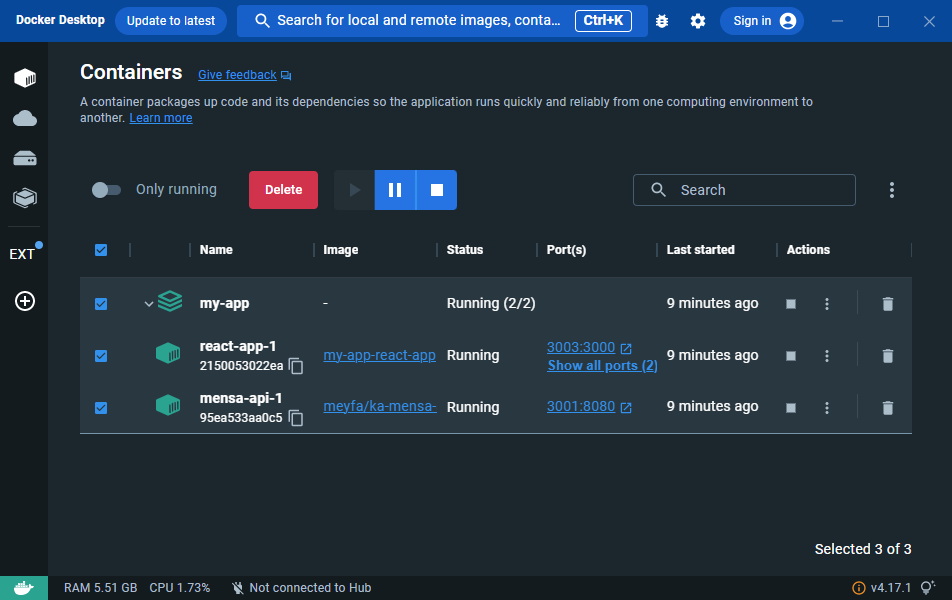
\includegraphics[width=\textwidth]{images/docker-desktop}}
	\caption{\label{fig-docker-desktop} Docker Desktop Screenshot}
\end{figure}

%%%%%%%%%%%%%%%%%%%%%%%%%%%%%%%%%%%%%%%%%%%%%%%%%%%%%%%%%%%%%%%%%%%%%%%%%%%%%%%
